\documentclass[12pt]{article}

\usepackage[T1]{fontenc} \usepackage[icelandic]{babel}
\usepackage{latexsym,amssymb,amsmath}
\usepackage{pgfplots}
\usepackage{float}
\usepackage[absolute,overlay]{textpos}
\newcounter{marknumber}
\pgfplotsset{
    error bars/every nth mark/.style={
        /pgfplots/error bars/draw error bar/.prefix code={
            \pgfmathtruncatemacro\marknumbercheck{mod(floor(\themarknumber/2),#1)}
            \ifnum\marknumbercheck=0
            \else
                \begin{scope}[opacity=0]
            \fi
        },
        /pgfplots/error bars/draw error bar/.append code={
            \ifnum\marknumbercheck=0
            \else
                \end{scope}
            \fi
            \stepcounter{marknumber}    
        }
    }
}
\usepackage{graphicx}
\graphicspath{ {./} }
\usepackage{hyperref, color}
\hypersetup{
    colorlinks=true,
    linktoc=all,
    linkcolor=blue,
}

\title{verklegt 5}
\author{mss32 }
\date{March 2022}

\begin{document}


\centerline{\bf \Huge EÐL207G Verkefni 5 Brotstuðull og ljóshraði}
\centerline{\bf Mikael Sævar Scheving Eggertsson, Torfi Þorgrímsson}

\centerline{\bf \large }

\tableofcontents
\newpage

\section{Inngangur}


\section{Tilraun}
\subsection{}

\setlength{\parindent}{0pt}

%2.1


\begin{center}
    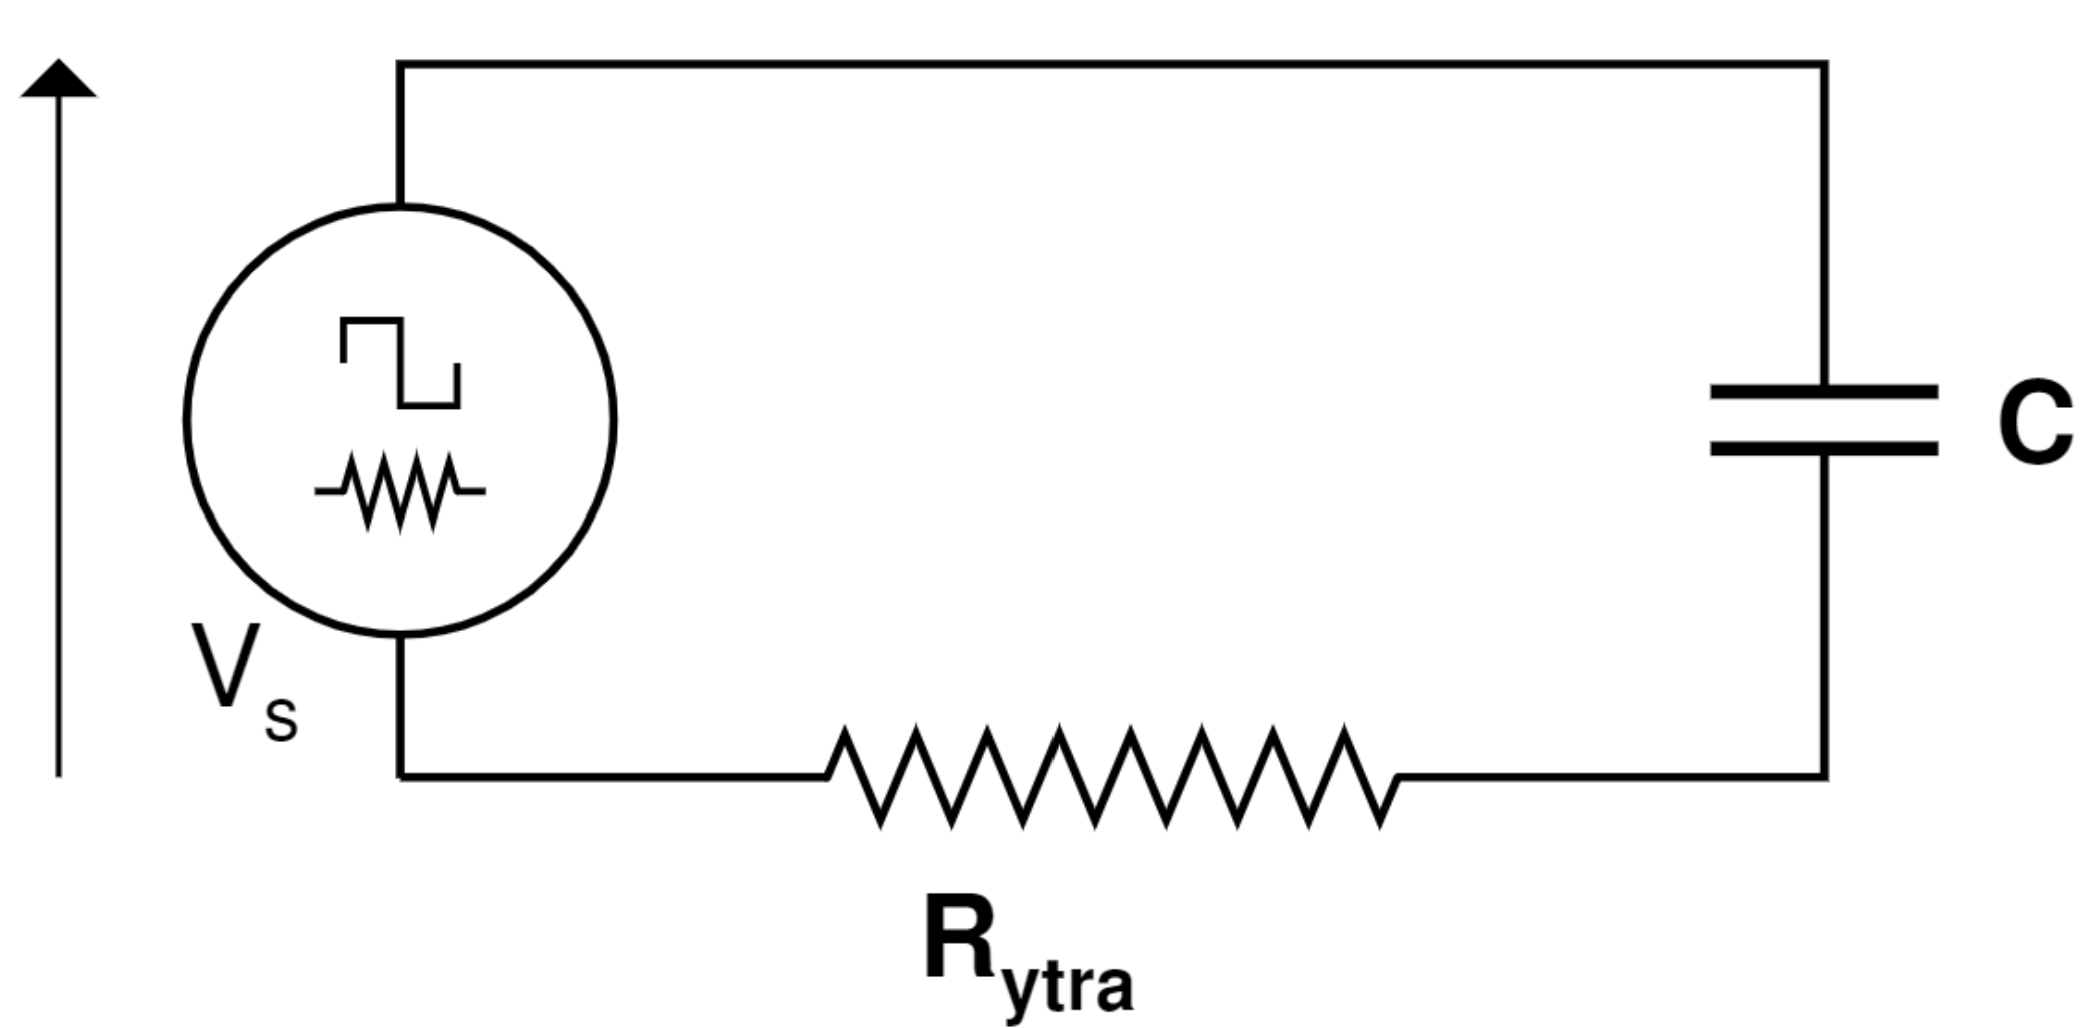
\includegraphics[scale=0.4]{mynd1}

Mynd 1 jpg jp
\end{center}

\textbf{Stutt lýsing:}


Speglum og grænum laser er stillt upp eins og á mynd 1, við það er hægt að sjá ráfur á spegli D frá sjónarhorni E. 
Hægt er að færa spegil D með vogarstöng sem er tengd við míkrómæli með hlutfallið 1:5. Með því að snúa míkrómælinum
færist spegillinn og bylgjunar á honum. Með því að telja bylgjur sem fara yfir fastann punkt í sjónarsviðinu er 
hægt að reikna út bylgjulengd laserins með jöfnu (2)



\textbf{Gildi notuð:}
\bigskip

 
 $v$ er hraði
 
 
 $n$ er brotstuðull
 
 
 $c$ er ljóshraði 
 

 $g$ er  gírstuðull vogstangarinnar
 

$x$ fjarlægð lesin á míkrómæli

 
 $\lambda$ er bylgjulengd
 
 
 $N$ er fjöldi ráka


 $z$ er feril spegils
 
 
 \bigskip


\textbf{Jöfnur notaðar:}
\bigskip
$ z=gx $ (1)


$N = \dfrac{z}{(\lambda/2)}$ (2)
\bigskip


\textbf{Mæld gidli:}

\begin{table}[H]
    \begin{tabular}{|c|c|c|c|c|}
    Mæling & $N$ & $x [m]$ & $gx=z [m]$ & $\lambda [m]$\\
    \hline
    1 & 100 & 180e-6 & 36e-6 & 720e-9 \\
    \hline
    2 & 94 & 120e-6 & 24e-6 & 510e-9 \\
    \end{tabular}
\end{table}

\subsection{}
% 2.2 

\textbf{Stutt lýsing:}
\bigskip

Á ljósleðinni úr sömu spegla uppsetningunni og í tilraun 1 er komið fyrir hylki á milli ADA ferilsins. 
Sá hylki hefur lengdina 50.0 ± 0.5 mm og er hægt að dæla inn og út einhverri gastegund. Komið er fyrir 
tveimur glerjum að sömu gerð og gluggarnir á hylkinu í ACA ferlinum til að tryggja að báðar leiðir séu
að öðru leyti eins. Við hylkið eru þrír stútar sem tengjast við loftdælu, þrýstingsmæli og andrúmsloftinu
í gegnum lokukerfi. Með því að hleypa lofti út hægt og rólega er hægt að telja hversu margar rákir færast
yfir fastann punkt. Með fjölda ráka fyrir ákveðna breytingu í þrýstingi, og gildi úr tilraun 1 er 
hægt að reikna brotstuðulinn með jöfnu (4). 
\bigskip

\textbf{Gildi notuð:}

\bigskip
$L$ er lengd gas hylkis


$M$ er fjöldi taldna ráka miðað viðað við fastann punkt


$f$ er tíðni ljósbylgjunar


$\Delta p$ er þrýstingsbreyting


$dM$ er rákafjöldi sem fer framhjá ákveðnum punkt í sjónarsviðinu   

\bigskip

\textbf{Jöfnur notaðar:}
\bigskip

$n = \frac{c}{v} =  \frac{f \lambda_0}{f \lambda} = \frac{ \lambda_0}{ \lambda}  $ (3)
\bigskip


$ n = 1+ \frac{\lambda_0 k}{2L}p$ (4)
\bigskip


$dM(\Delta p) = k (\Delta p) $ (5)
\bigskip

\textbf{Mæld gidli:}

\begin{table}[H]
    \begin{tabular}{|c|c|c|c|c|c|c|}
    $p[cmHg]$ & 70 & 50 & 40 & 30 & 20 & 10\\
    \hline
    $M$ & 0 & 12 & 16 & 21 & 26 & 32 \\
    \end{tabular}
\end{table}

$\Delta p = 60 cmHg$
\bigskip

$dM = 32$
\bigskip

$k=\dfrac{dM}{\Delta p} = (533+\frac{1}{3})e-3$
\bigskip

\begin{table}[H]
    \begin{tabular}{|c|c|c|}
    Mæling & $n-1$ \\
    \hline
    1 & 2.91840e-6 \\
    \hline
    2 & 2.06978e-6 \\
    \end{tabular}
\end{table}

 \bigskip


\section{Niðurstaða}

\subsection{Tilraun 1}
Niðurstöðurnar úr útreikningunum ásamt skekkjumörkum falla innann við líkanið okkar sem er bylgjulengd á bilinu 495nm-570nm. Þótt það er ekki hægt segja nákvæmlega hvaða gildi er á bylgjulengdinni þá getum við sagt að laserinn er grænn. 



\subsection{Tilraun 2}
Niðurstaðan er að brotstuðulinn breytist með þrýsting, sem er niðurstaðan sem við vorum að leitast eftir. Líklegasta ástæðan er að fyrir hærri þrýsting þá er meira gas fyrir ljósið til að rekast á. 


\end{document}


